\begin{multicols}{2}
\section{Evidence Provenance and the Positioning Search}
\label{app:sources}
\setcounter{table}{0}
\setcounter{figure}{0}

Sources serve two roles. Collected practice sources supplied the mechanisms generalized into the 79 patterns. Later literature searches located related work without changing those patterns or the Specification. The practice sources are 101 source pages, which record 91 distinct documents. Table~\ref{tab:practice-sources} names the documents behind each pattern. The two source sets share one work: ISO/IEC/IEEE 15288 supplied \hyperlink{gp-16}{GP-16} and is also cited as related work.

\subsection{Practice sources by pattern}

Collection agents recorded each source page with the document they read and the organization or practitioner that the document credits with the practice. Most of the documents are web pages: agency handbooks and procedural requirements, standards summaries, engineering blogs, product documentation, interviews, and preprints. Some pages report the practice of an organization through a second party. For example, a tool vendor describes the SpaceX design process, and a trade publication describes a Boeing program. For such a page, the table names the organization whose practice is described and cites the document that describes it.

Web pages change and move, so each bibliography entry gives the address that was read, the date the source page entered the project record, and a copy in the Wayback Machine of the Internet Archive. I used the capture nearest to that date. Three documents had no capture, and I requested one on 2026-09-25. Two documents have no archived copy: an access-restricted standard and a document whose address now leads to a landing page.

A pattern that absorbed merged candidates lists their sources as well, so one pattern can cite several documents. The table records attribution only. It does not rate the sources, and it does not confirm that an organization follows the practice today.
\end{multicols}

\begingroup
\renewcommand{\arraystretch}{0.9}
\footnotesize
\begin{longtable}{@{}l p{0.36\textwidth} p{0.30\textwidth} p{0.20\textwidth}@{}}
\caption{Practice sources per pattern. The attribution follows the source pages of Generalized Patterns; the cited entries give the address read, the access date, and the archived copy.}
\label{tab:practice-sources} \\
\toprule
Pattern & Name & Practice attributed to & Documents \\
\midrule
\endfirsthead%
\multicolumn{4}{@{}l}{\tablename~\thetable{} (continued)} \\
\toprule
Pattern & Name & Practice attributed to & Documents \\
\midrule
\endhead%
\hyperlink{gp-01}{GP-01} & Versioned execution plans as the system of record & OpenAI & \citep{ps-openai-harness} \\
\hyperlink{gp-02}{GP-02} & Verify-and-record iteration discipline & Geoffrey Huntley & \citep{ps-huntley-ralph} \\
\hyperlink{gp-03}{GP-03} & The binding work-unit document & Kent Beck & \citep{ps-beck-augmented} \\
\hyperlink{gp-04}{GP-04} & Structured work record over fragile prose & Steve Yegge & \citep{ps-yegge-beads} \\
\hyperlink{gp-05}{GP-05} & Typed dependencies and derived readiness & Steve Yegge & \citep{ps-beads-readme} \\
\hyperlink{gp-06}{GP-06} & Documents as the sole coordination medium & Microsoft Research & \citep{ps-msr-corpgen} \\
\hyperlink{gp-07}{GP-07} & Product-anchored decomposition with a dictionary & NASA & \citep{ps-nasa-wbs} \\
\hyperlink{gp-08}{GP-08} & Purpose-defined units with owner and binary verification & SpaceX & \citep{ps-singh-billofdesign} \\
\hyperlink{gp-09}{GP-09} & System-level contracts before component detail & SpaceX & \citep{ps-singh-fivetips} \\
\hyperlink{gp-10}{GP-10} & Work-unit sizing & Steve Yegge & \citep{ps-yegge-revenge} \\
\hyperlink{gp-11}{GP-11} & The verifiable task as the unit of work & Amjad Masad (Replit); Cognition & \citep{ps-masad-selfdriving,ps-cognition-devin} \\
\hyperlink{gp-12}{GP-12} & Blast-radius-bounded work units & Peter Steinberger & \citep{ps-steinberger-talk} \\
\hyperlink{gp-13}{GP-13} & Nested levels of intent, each with acceptance criteria & Birgitta B\"ockeler (Thoughtworks) & \citep{ps-bockeler-loops} \\
\hyperlink{gp-14}{GP-14} & Milestone decomposition with repair-before-progression & OpenAI & \citep{ps-openai-longhorizon} \\
\hyperlink{gp-15}{GP-15} & Numbered design generations & SpaceX & \citep{ps-sesnic-raptor} \\
\hyperlink{gp-16}{GP-16} & Four recursive process groups & ISO/IEC/IEEE 15288 & \citep{ps-jama-15288} \\
\hyperlink{gp-17}{GP-17} & Specification-first, self-contained contract before execution & Anthropic & \citep{ps-anthropic-bestpractices} \\
\hyperlink{gp-18}{GP-18} & Human-approved plan gate & Anthropic & \citep{ps-anthropic-bestpractices} \\
\hyperlink{gp-19}{GP-19} & The specification is the durable alignment artifact & Sean Grove (OpenAI) & \citep{ps-grove-newcode} \\
\hyperlink{gp-20}{GP-20} & Unique, verifiable obligation statements & NASA & \citep{ps-nasa-npr7123} \\
\hyperlink{gp-21}{GP-21} & Fixed structure for obligation statements & ISO/IEC/IEEE 29148 & \citep{ps-ieee-29148} \\
\hyperlink{gp-22}{GP-22} & Obligation hierarchy with fixed record attributes & ISO/IEC/IEEE 29148 & \citep{ps-reqview-29148,ps-iso-29148} \\
\hyperlink{gp-23}{GP-23} & Named owner for every obligation & SpaceX & \citep{ps-sesnic-starbase} \\
\hyperlink{gp-24}{GP-24} & Constraint provenance marking & SpaceX & \citep{ps-singh-fivetips} \\
\hyperlink{gp-25}{GP-25} & Verification method assigned at authoring & ISO/IEC/IEEE 15288 & \citep{ps-jama-15288} \\
\hyperlink{gp-26}{GP-26} & One fixed lens for every interface & NASA & \citep{ps-nasa-seh-appl} \\
\hyperlink{gp-27}{GP-27} & Public contract, private design, co-updated realization & Hartwig Grabowski & \citep{ps-grabowski-specgrowth} \\
\hyperlink{gp-28}{GP-28} & Adversarial expansion of the contract & Berkeley AI Research & \citep{ps-parameswaran-bair} \\
\hyperlink{gp-29}{GP-29} & Named key design parameters, no added coordination roles & SpaceX & \citep{ps-altium-spacex} \\
\hyperlink{gp-30}{GP-30} & Artifact-gated phase sequence & GitHub & \citep{ps-delimarsky-speckit} \\
\hyperlink{gp-31}{GP-31} & Done is a checkable criterion, never self-assessment & Anthropic & \citep{ps-anthropic-bestpractices} \\
\hyperlink{gp-32}{GP-32} & Verifiability governs what may be delegated & Andrej Karpathy & \citep{ps-karpathy-verifiability} \\
\hyperlink{gp-33}{GP-33} & Acceptance check authored before work begins & Simon Willison & \citep{ps-willison-redgreen} \\
\hyperlink{gp-34}{GP-34} & Establish the verification baseline before changing anything & Simon Willison & \citep{ps-willison-firsttests} \\
\hyperlink{gp-35}{GP-35} & Durable verification corpus & Hamel Husain; Google; Jason Liu & \citep{ps-husain-evals,ps-google-agentscli,ps-liu-context} \\
\hyperlink{gp-36}{GP-36} & Layered verification mirroring decomposition & AWS AI & \citep{ps-aws-agentic} \\
\hyperlink{gp-37}{GP-37} & Verification correspondence for every decomposition level & INCOSE & \citep{ps-wayne-vee} \\
\hyperlink{gp-38}{GP-38} & Governing verification plan & IEEE & \citep{ps-futureskill-1012,ps-ansi-1012} \\
\hyperlink{gp-39}{GP-39} & Recorded criticality class determines rigor & NASA; INCOSE; NASA IV\&V Program & \citep{ps-nasa-npr7150,ps-jama-incose,ps-nasa-ivv} \\
\hyperlink{gp-40}{GP-40} & Generator and verifier are independent & Itamar Friedman (Qodo) & \citep{ps-friedman-qodo} \\
\hyperlink{gp-41}{GP-41} & Acceptance artifacts are inviolable & Kent Beck & \citep{ps-beck-augmented,ps-orosz-beck} \\
\hyperlink{gp-42}{GP-42} & Every contract clause linked to its check & Sean Grove (OpenAI) & \citep{ps-grove-newcode} \\
\hyperlink{gp-43}{GP-43} & Structure outputs for verification & Hamel Husain & \citep{ps-husain-evalsmell} \\
\hyperlink{gp-44}{GP-44} & Evidence before, verification after, every phase & Pardis Taghavi and Santosh Bhavani & \citep{ps-taghavi-speckit} \\
\hyperlink{gp-45}{GP-45} & Linked stage checks across production & TSMC & \citep{ps-tsmc-epo,ps-tsmc-ar2014} \\
\hyperlink{gp-46}{GP-46} & Model-based verification before costly realization & Boeing & \citep{ps-hannover-boeing} \\
\hyperlink{gp-47}{GP-47} & Reference realization with drift detection & Birgitta B\"ockeler (Thoughtworks) & \citep{ps-bockeler-anchoring} \\
\hyperlink{gp-48}{GP-48} & Durable execution records & Armin Ronacher & \citep{ps-ronacher-agentic} \\
\hyperlink{gp-49}{GP-49} & Event-based gates with recorded closure & NASA & \citep{ps-nasa-npr7123} \\
\hyperlink{gp-50}{GP-50} & Approved baselines at defined levels & NASA; Aerospace industry practice & \citep{ps-nasa-seh-cm,ps-zheng-baseline} \\
\hyperlink{gp-51}{GP-51} & One controlled change gate & NASA & \citep{ps-nasa-seh-cm} \\
\hyperlink{gp-52}{GP-52} & One configuration status ledger & NASA & \citep{ps-nasa-seh-cm} \\
\hyperlink{gp-53}{GP-53} & Explicit deviation matrix & NASA & \citep{ps-nasa-npr7123} \\
\hyperlink{gp-54}{GP-54} & Separate structural and behavioral change & Kent Beck & \citep{ps-beck-augmented} \\
\hyperlink{gp-55}{GP-55} & Traceability as a structural property & Thorsten Schlath\"olter & \citep{ps-schlatholter-reqtocode} \\
\hyperlink{gp-56}{GP-56} & Bidirectional traceability, verification and validation separate & NASA & \citep{ps-nasa-seh-app} \\
\hyperlink{gp-57}{GP-57} & Versioned input lineage for reproducible results & Lockheed Martin & \citep{ps-lakefs-lockheed} \\
\hyperlink{gp-58}{GP-58} & The realization system is traced like the product & Boeing & \citep{ps-boeing-thread} \\
\hyperlink{gp-59}{GP-59} & One canonical source of truth per concern & Amjad Masad (Replit); Airbus & \citep{ps-masad-selfdriving,ps-airbus-collab} \\
\hyperlink{gp-60}{GP-60} & Numbered, immutable decision records & Michael Nygard; Andrew Harmel-Law; ThoughtWorks; ADR community; MADR maintainers; Olaf Zimmermann & \citep{ps-nygard-adr,ps-harmellaw-scaling,ps-thoughtworks-adr,ps-adr-github,ps-madr,ps-zimmermann-anydr} \\
\hyperlink{gp-61}{GP-61} & Continuous risk register with documented human acceptance & NASA & \citep{ps-nasa-swe086} \\
\hyperlink{gp-62}{GP-62} & Failure closure by numbered corrective actions & SpaceX and the FAA & \citep{ps-faa-starship,ps-smith-oft2} \\
\hyperlink{gp-63}{GP-63} & Invariants as mechanically checkable constraints & OpenAI & \citep{ps-openai-harness} \\
\hyperlink{gp-64}{GP-64} & Declared executor scope & Guillermo Rauch (Vercel); Anthropic & \citep{ps-brandom-rauch,ps-anthropic-subagents} \\
\hyperlink{gp-65}{GP-65} & Disposable executors, durable work, structural boundaries & Microsoft and GitHub & \citep{ps-microsoft-squad} \\
\hyperlink{gp-66}{GP-66} & Directives as controlled artifacts & Dex Horthy (HumanLayer) & \citep{ps-horthy-factor2} \\
\hyperlink{gp-67}{GP-67} & Delegated work stays isolated behind a summary interface & Anthropic & \citep{ps-anthropic-context} \\
\hyperlink{gp-68}{GP-68} & One governing-principles document & GitHub; JPL & \citep{ps-github-speckit,ps-jpl-d17868,ps-jpl-principles} \\
\hyperlink{gp-69}{GP-69} & Governance content discipline & Roland Huss; Cursor; AWS AI; Geoffrey Huntley & \citep{ps-huss-agentsmd,ps-cursor-rules,ps-aws-agentic,ps-huntley-loom} \\
\hyperlink{gp-70}{GP-70} & Short entry point into a versioned documentation tree & OpenAI; Geoffrey Huntley & \citep{ps-openai-harness,ps-huntley-groundhog} \\
\hyperlink{gp-71}{GP-71} & Governance bound to component boundaries & OpenAI, Cursor, LangChain, Mistral AI & \citep{ps-agentsmd,ps-openai-agentsmd,ps-cursor-rules,ps-langchain-deepagents,ps-mistral-agents} \\
\hyperlink{gp-72}{GP-72} & Placement and naming are declared structure & Anthropic & \citep{ps-anthropic-context} \\
\hyperlink{gp-73}{GP-73} & Documentation lives on the artifact it governs & Cyrille Martraire; Armin Ronacher & \citep{ps-stenberg-livingdoc,ps-ronacher-agentic} \\
\hyperlink{gp-74}{GP-74} & One named owner plus a standing flaw-checker & Eugene Yan & \citep{ps-yan-mechanisms} \\
\hyperlink{gp-75}{GP-75} & Durable human breakpoints in the control flow & Dex Horthy (HumanLayer) & \citep{ps-horthy-factor8} \\
\hyperlink{gp-76}{GP-76} & Human-owned contract, machine-readable surfaces & Andrej Karpathy & \citep{ps-karpathy-sequoia} \\
\hyperlink{gp-77}{GP-77} & Reusable task definitions with postconditions and prohibitions & Cognition; LangChain & \citep{ps-cognition-playbooks,ps-langchain-context} \\
\hyperlink{gp-78}{GP-78} & One registry; unregistered does not exist & OpenAI & \citep{ps-openai-cookbook} \\
\hyperlink{gp-79}{GP-79} & Why--What--How document skeleton & Eugene Yan & \citep{ps-yan-designdocs} \\
\bottomrule
\end{longtable}
\endgroup

\begin{multicols}{2}
\subsection{Mechanism attribution by family}

Table~\ref{tab:family-sources} groups the located literature by mechanism family. A source found for two families appears in both rows, so the column total exceeds the 1,277 unique sources found on pattern items. The counts describe retrieval, not the strength of support for a pattern.

The family labels include representative sources for the mechanisms or their research context. These citations do not establish the effectiveness of a whole family. No verified external source was selected for the reusable-procedure family.

The table groups sources by the pattern ranges shown, excludes control items, and counts each distinct source once within a family. Figure~\ref{fig:family-domains} counts by the same rules and shows the sources of each family in all domains and all citation states. Search agents assigned the source domains and citation states. Read-verified means that an agent recorded a full-text check of the source identity, cited claim, population, and limitations. It does not record human verification.
\end{multicols}

\begingroup
\renewcommand{\arraystretch}{0.9}
\footnotesize
\begin{longtable}{@{}p{0.24\textwidth} l r r r p{0.28\textwidth}@{}}
\caption{Located literature per mechanism family. Sources are unique citations found for at least one form of the family; a source found for forms of two families appears in both rows. Citation states are the search agents' recorded assessments. Leading domains exclude unclassified sources.}
\label{tab:family-sources} \\
\toprule
Family and representative sources & Forms & \# & Sources & Read-verified & Leading domains \\
\midrule
\endfirsthead%
\multicolumn{6}{@{}l}{\tablename~\thetable{} (continued)} \\
\toprule
Family and representative sources & Forms & \# & Sources & Read-verified & Leading domains \\
\midrule
\endhead%
Durable work record \citep{provdm2013} & \hyperlink{gp-01}{GP-01} to \hyperlink{gp-06}{GP-06} & 6 & 141 & 45 & software and computing 50; medicine and patient safety 24 \\
Decomposition \citep{parnas1972} & \hyperlink{gp-07}{GP-07} to \hyperlink{gp-16}{GP-16} & 10 & 211 & 72 & software and computing 76; organization science and management 26 \\
Contract and obligation \citep{meyer1992} & \hyperlink{gp-17}{GP-17} to \hyperlink{gp-30}{GP-30} & 14 & 261 & 74 & software and computing 79; organization science and management 31 \\
Verification and acceptance \citep{cruz2023} & \hyperlink{gp-31}{GP-31} to \hyperlink{gp-49}{GP-49} & 19 & 323 & 92 & software and computing 119; aviation and aerospace 34 \\
Configuration control \citep{iso15288} & \hyperlink{gp-50}{GP-50} to \hyperlink{gp-54}{GP-54} & 5 & 90 & 21 & aviation and aerospace 24; software and computing 22 \\
Traceability and lineage \citep{gotel1994} & \hyperlink{gp-55}{GP-55} to \hyperlink{gp-59}{GP-59} & 5 & 73 & 11 & software and computing 25; manufacturing and quality 9 \\
Decision record \citep{manteuffel2018} & \hyperlink{gp-60}{GP-60} & 1 & 11 & 4 & software and computing 7; human factors 1 \\
Risk and failure \citep{parasuraman1997} & \hyperlink{gp-61}{GP-61} to \hyperlink{gp-62}{GP-62} & 2 & 33 & 8 & medicine and patient safety 9; organization science and management 6 \\
Executor boundary \citep{saltzer1975} & \hyperlink{gp-63}{GP-63} to \hyperlink{gp-67}{GP-67} & 5 & 108 & 31 & software and computing 43; organization science and management 11 \\
Governance document \citep{chatlatanagulchai2025readme,gloaguen2026} & \hyperlink{gp-68}{GP-68} to \hyperlink{gp-73}{GP-73} & 6 & 74 & 23 & software and computing 23; organization science and management 7 \\
Role and authority \citep{parasuraman2000} & \hyperlink{gp-74}{GP-74} to \hyperlink{gp-76}{GP-76} & 3 & 24 & 15 & software and computing 6; aviation and aerospace 5 \\
Reusable procedure (no source selected) & \hyperlink{gp-77}{GP-77} to \hyperlink{gp-79}{GP-79} & 3 & 38 & 9 & software and computing 15; standards and specifications 4 \\
\bottomrule
\end{longtable}
\endgroup

\begin{figure}[htbp]
\centering
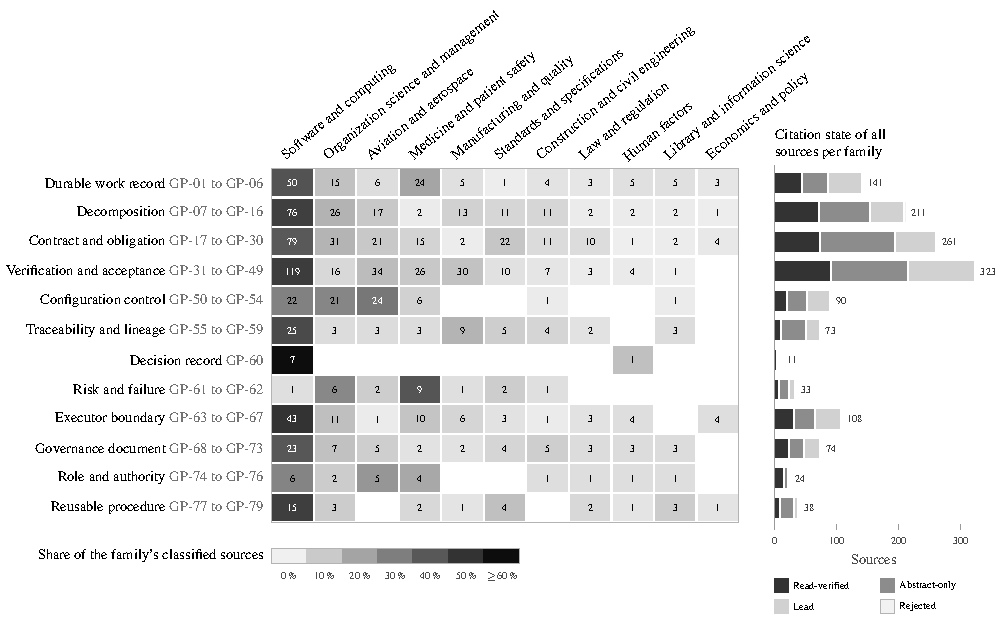
\includegraphics[width=\textwidth]{figures/f11/f11-literature-domains.pdf}
\caption{Located literature per mechanism family, by source domain and by citation state. On the left, each number counts the family's sources in one domain, and the shade gives that count as a share of the family's classified sources. The left panel does not show unclassified sources, and an empty cell is a zero count. On the right, each bar splits all sources of the family by citation state, with the total at its end. The counting rules are those of Table~\ref{tab:family-sources}: a source found for two families counts in both rows, and control items are excluded. Search agents assigned the domains and the citation states, and no human verification is recorded.}
\label{fig:family-domains}
\end{figure}

\begin{multicols}{2}
\subsection{Search procedure and limits}

The first search worked outward from mechanism families, since several patterns can share one research base. A later audit used a protocol fixed before that pass and searched all 79 patterns and the control items again. It recorded the queries, sources, and citation states. Deduplication matched source identifiers and titles, with conflicting matches or states recorded for review.

Only sources marked Read-verified could support result claims. Abstract-only sources could establish a work's existence and topic. Unchecked leads could support no substantive citation. Human checking against a primary record remained a separate requirement before bibliography acceptance.

The first pass had no registered protocol or fixed query set. The later audit agents used one general search engine to reach publisher pages, preprint archives, and institutional records. They could not query the separate discovery services named in the protocol directly. The source set therefore depends on that search engine's retrieval.

The audit allowed eight discovery queries per item. Twelve calls across nine items exceeded that limit, with reasons recorded. Sources found only through those calls were excluded from the result files. The planned re-search of 39 merged candidates and blind re-classification of 101 screening rejects were not completed.

\subsection{Agreement between repeated searches}

Duplicate dispatch produced paired searches for \hyperlink{gp-61}{GP-61} through \hyperlink{gp-69}{GP-69} under the same model, protocol, and date. Source matching used DOI, then arXiv identifier, then normalized title. Across 18 directed comparisons, 19 of 120 opened sources were found in the paired run, or 15.8 per cent.

This is observed identifier-based overlap, not a recall estimate for the literature. Different identifiers can hide a match: one recorded work appeared with a DOI in one run and as an unidentified lead in the other. These paired runs show that the retrieved source list was not stable. The map records what the searches found, not the limits of the available literature.

\subsection{The withdrawn rating instrument}

The method for rating literature support was withdrawn after its controls failed to separate relevant evidence from analogy reliably; the paper retains source attribution without support scores.

The source counts in Table~\ref{tab:family-sources} describe what the searches found. They do not measure how strongly the literature supports a pattern or how completely the searches cover a field.
\end{multicols}
